\subsection{Análisis de HW}

El circuito de prueba construido para este proyecto se subdivide en dos secciones importantes: el circuito de control y el de potencia. El primero de estos dos se puede observar en la figura \ref{circuito_control}.

\begin{figure}[H]
\centering
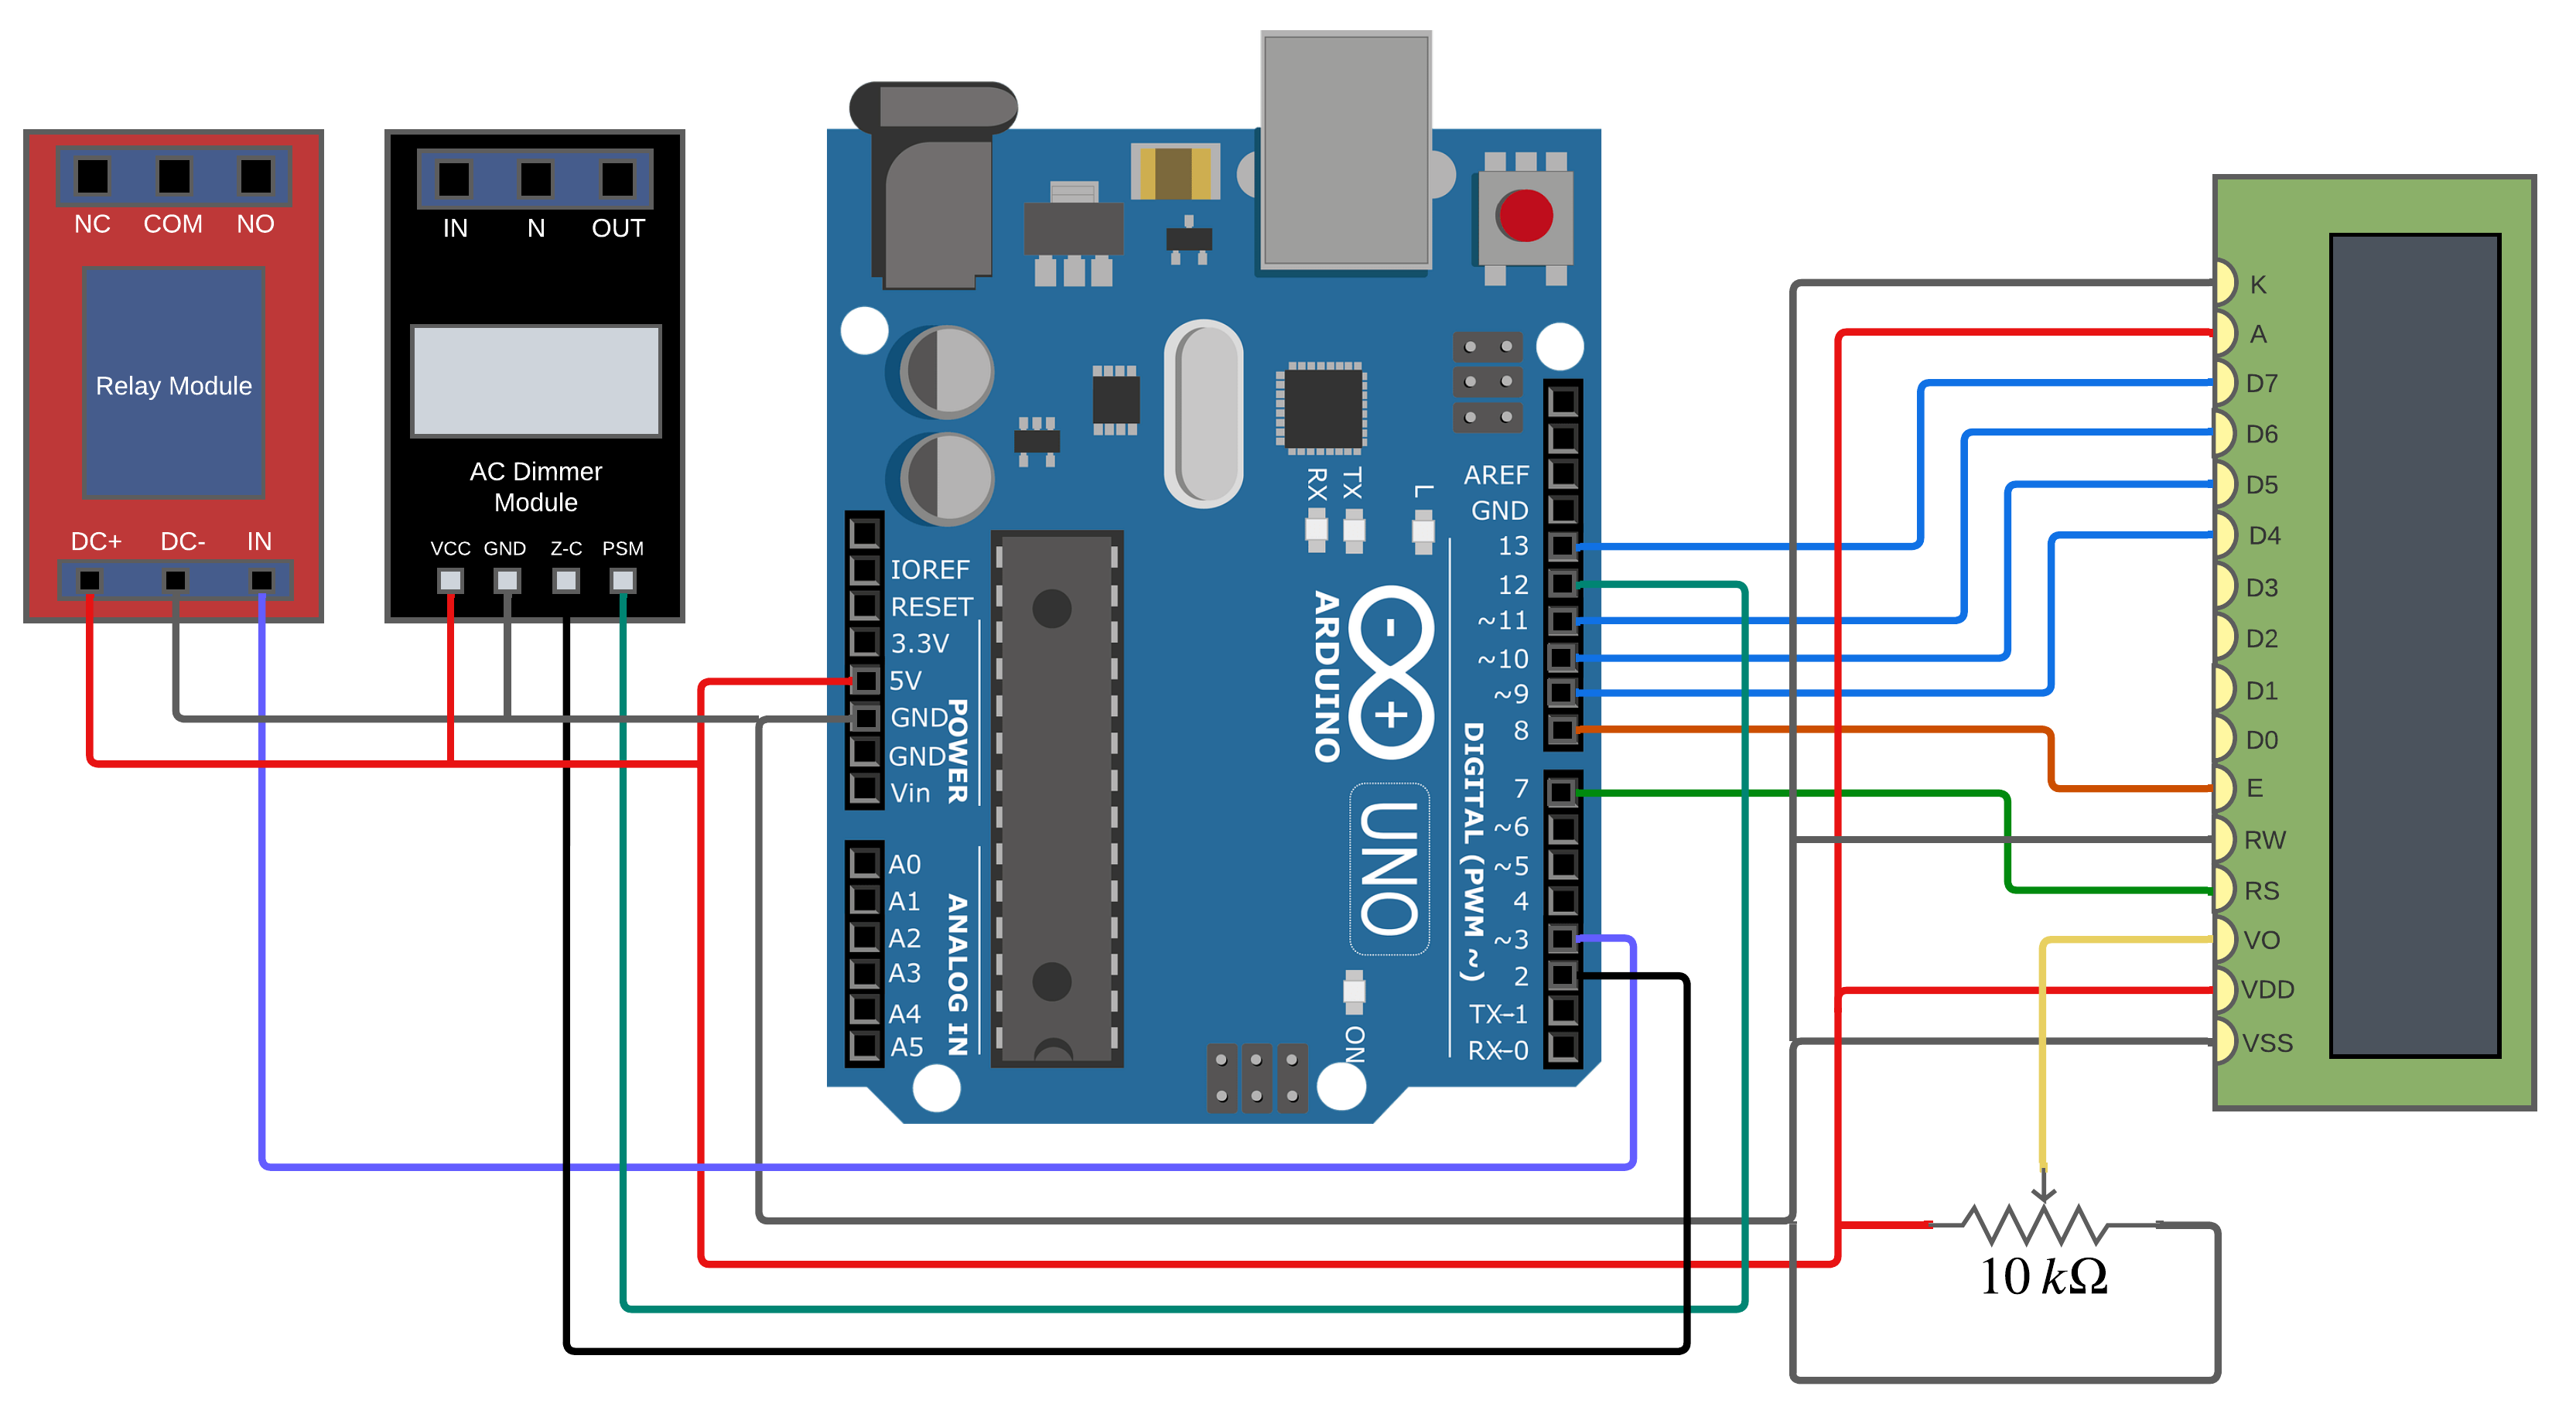
\includegraphics[scale=0.62]{./images/control.png} 
\caption{Diagrama del circuito de control}
\label{circuito_control}
\end{figure}

\vspace*{-0.3cm}

Por otra lado, la parte correspondiente al circuito de potencia se presenta en la figura \ref{potencia}.

\begin{figure}[H]
\centering
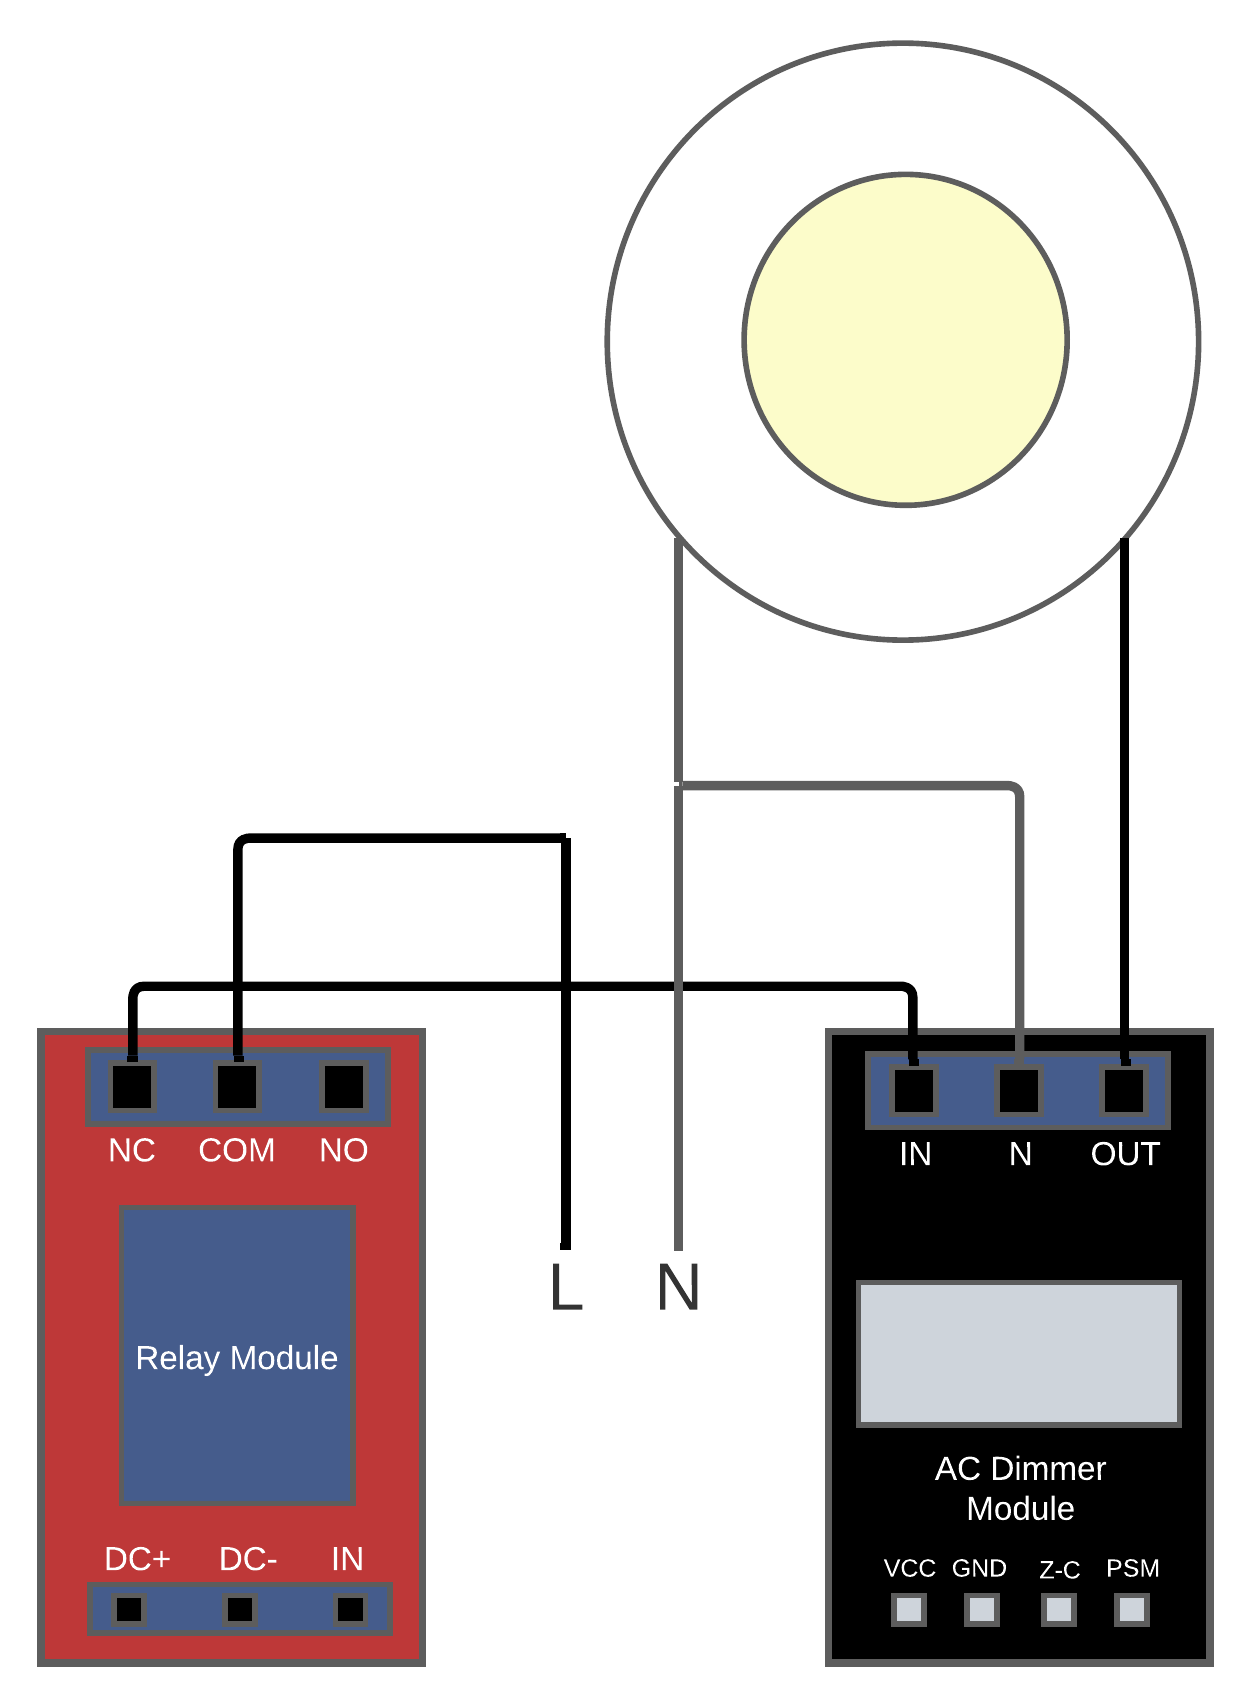
\includegraphics[scale=0.62]{./images/potencia.png} 
\caption{Diagrama del circuito de potencia }
\label{potencia}
\end{figure}

Con respecto al circuito de control, primeramente se sabe que la bobina del relé consume $90\,mA$ y necesita estar alimentada a $5\,V$ para operar correctamente. Al multiplicar estos últimos dos datos se puede determinar que la potencia consumida por el relé es de $450\,mW$. Por otra parte, la pantalla LCD 16x2 presenta un consumo máximo de $25\,mA$ y requiere de $5\,V$ para funcionar, por lo tanto, este componente consume aproximadamente $125\,mW$. En cuanto al módulo dimmer AC, se sabe que sus periféricos pueden operar adecuadamente a cualquier corriente menor a $10\,mA$. Además, este componente también está conectado a la fuente de tensión de $5\,V$ del Arduino UNO. Tomando en cuenta estos datos, se tiene que el módulo dimmer AC puede llegar a consumir hasta $50\,mW$. Al sumar todos los resultados anteriores, se tiene un consumo de potencia de $625\,mA$ por parte del circuito de control. 

Por el lado del circuito de potencia, el único el único elemento que presenta consumo de potencia es la resistencia de la bombilla incandescente. El valor de dicha potencia corresponde a un máximo de $100\,W$.

 \textbf{A continuación se presenta un link para accesar y ver un video de su correcto funcionamiento:}\\



\hspace{0.5mm}\url{https://drive.google.com/drive/folders/12DI6IFieF0CJ9Nj7iPxgw47PLW-znKQv?usp=sharing} 